\chapter{Internal Architecture}

\section{States}
%This section will explain the internal architecture of the launcher, this is every dependency inside the launcher.
Being able to launch an \girafapp[] as a specific guardian requires the user to interact such that the launcher knows which guardian the user represents.

Authentication was chosen, as each modulated child and guardian contains private data and therefore needs to be protected. QR-codes was chosen as means of authentication, as they provide a level of security.
An alternative to QR-codes could be a \emph{username-password} method, where each user have their own username, with an private password.
%The system is designed to have the two modes: guardian- and child mode\todo{ref to backlog}.
As explained in \autoref{backlog_childmode}\todo{tilfoej childmode til backlog}, 

The launcher is developed towards being a tool usable by both guardians and children e.g. the ``child mode'' feature, described in \autoref{backlog_childmode}\todo{tilfoej childmode til backlog}.

A username-password combination requires the user to remember their credentials, whereas some \autists[] have problems with it.

\myQuote{Some \autists[] can have problems remembering a username and password  -  Drazenko Banjak, educator at Egebakken.} \todo{Compare style to commen-rapport qoute}

QR-codes provides a physical way of storing the user credentials and allows for other users to take responsibility of the QR-code, such as a \guardian[] carrying a QR-code of a \autist[].

QR-codes can be scanned by a built-in camera on tablets and can be printed using standard paper and printer equipment. 

QR-codes are copyable, by e.g. a copymachine, and therefore must be kept away from untrusted users, if they should not be used by people for which they were not intended.

To sum up, QR-codes are chosen because of they improve usability, despite of their ability to be copied.\todo{Ulrik, er dette i orden?}



\begin{figure}[h]
	\centering
	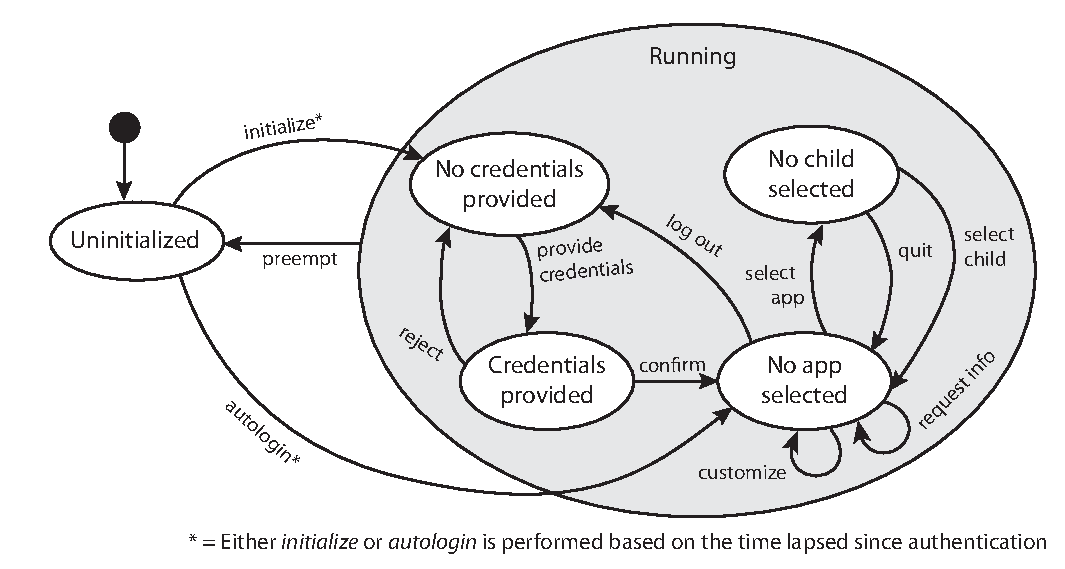
\includegraphics[width=1\textwidth]{gfx/statediagram.pdf}
	\caption{Flow diagram}
	\label{fig:flow_diagram}
\end{figure}

\autoref{fig:flow_diagram} shows the state of the launcher. The first three states handles the distinction between users which are allowed to access the launchable applications, and those who are not. \todo{indsaet ref til der hvor vi fandt ud af at vi skulle have authentication}


\section{Functionality}

\todo{thomas, read this}
\autoref{fig:design_diagram} shows the states divided into functionality groups, which describe a specific feature from the backlog.

%To specificy a more detailed design, the need for narrowing down the abstract states into features are required.
%The states are divided into feature groups, which can seen in \autoref{fig:design_diagram}.
%Each feature's functionality is defined by each outgoing action from the states the feature originates from. 

\begin{figure}[h]
	\centering
	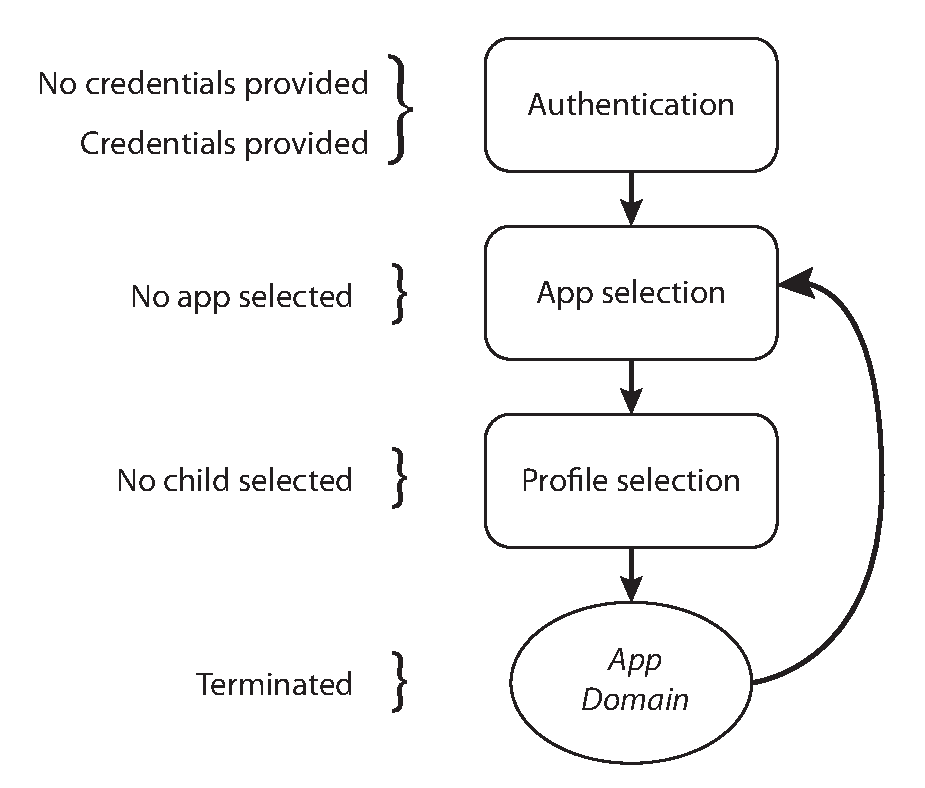
\includegraphics[width=1\textwidth]{gfx/design_diagram.pdf}
	\caption{Design diagram}
	\label{fig:design_diagram}
\end{figure}
\todo{Wombat og Parrot skal skrives med stort}

\subsection{Authentication}
\label{design:authentication}
The authentication functionality -- represented as the \nameref{backlog:authentication} feature in \autoref{backlog:authentication} -- is illustrated in \autoref{fig:authentication_design}. 
\begin{figure}[h]
	\centering
	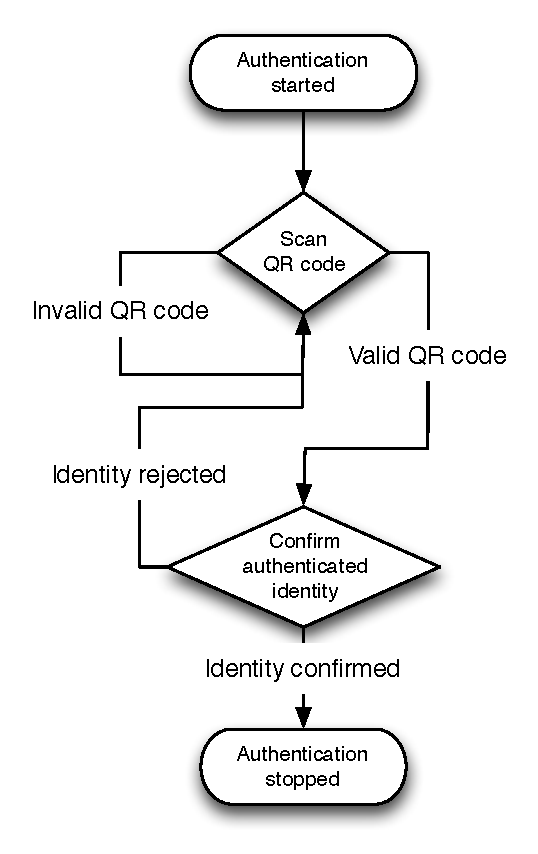
\includegraphics[width=0.5\textwidth]{gfx/authentication_design.pdf}
	%\caption{Features of the Authentication feature}
	\caption{Flowchart of the authentication functionality}
	\label{fig:authentication_design}
\end{figure}

\noindent The authentication consists of two steps:

\begin{enumerate}
	\item validating
	\item confirmation
\end{enumerate}

The validation step consists of scanning the provided QR-code. If valid, the user is asked to confirm the scanned identity, or reject if needed. The user is not allowed to proceed if the QR-code is unvalid.

Confirmation is chosen, in order to avoid authentications where a user uses a QR-code which is not the one the user thought it was.

%Upon scanning a QR-code, there is two possible outcomes: The QR-code is invalid, as the credentials are not recognized, or the QR-code contains credentials which are recognized.
%In case of the QR-code being valid, the process then enters it second step. The second step consist of the user needs to confirm the identity, or reject if identity represented on the system does not match the user's identity. 

\subsection{App management}
\label{design:app_manangement}
The app management functionality is illustrated in \autoref{fig:appmanagement_design}. 
\begin{figure}[h]
	\centering
	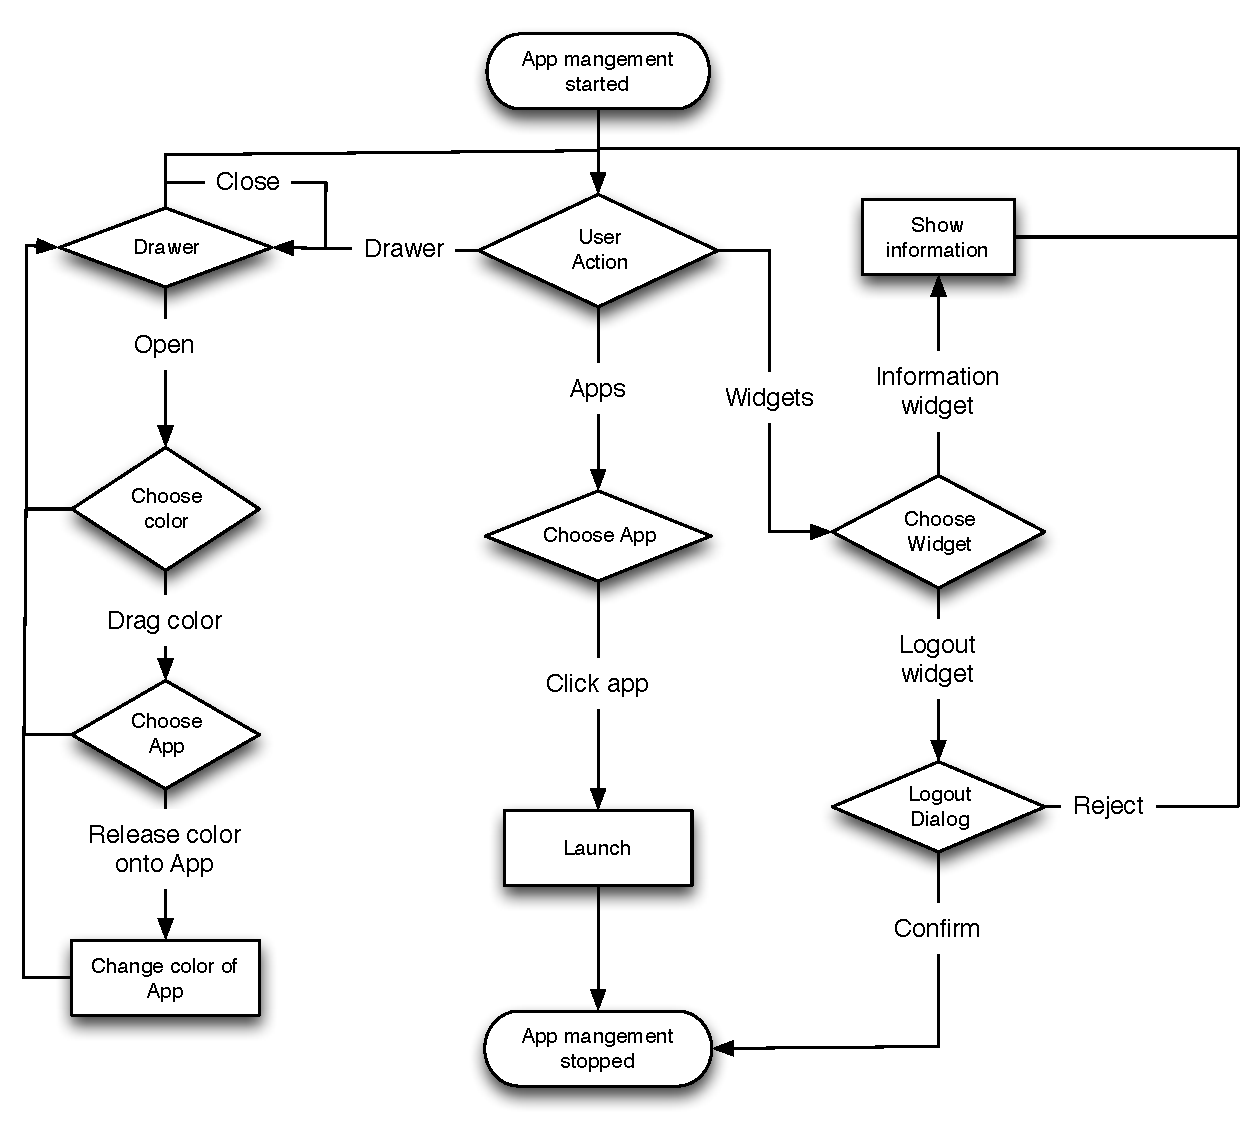
\includegraphics[width=1\textwidth]{gfx/appmanagement.pdf}
	\caption{Features of the App management feature}
	\label{fig:appmanagement_design}
\end{figure}
User interaction is the initial step fof the app management functionality, and can be one of the three interactions:

\begin{enumerate}
	\item Change app settings
	\item Launch app
	\item Request information
\end{enumerate}

%User action is the initial step of the app management feature, and controls the interaction with the user.
%One of the actions the user is able to make, is to change settings regarding the current authenticated user's apps.
The user does that by interacting with the drawer \todo{insert ref to preanalysis}.
The drawer can be opened or closed.
The closed state is when the drawer is sled all the way to the left.
The open state is when the drawer is when is not sled all the way to the left, and is below or at its maximum span.
When the drawer is opened, it is possible to change a color of an app.
This is done by dragging a color from the color table, onto an app and releasing in order to make the app change color.
The system can then return to the initial state.

Another action the user is able to make, is to retrieve information regarding the system.
After the information have been shown to the user, the user returns to the initial state.
The last action the user is able to make from the initial state is to launch an app.
This is done by the user clicking on the app, and then app management process is over.

\subsection{Profile selection}
The profile selection feature is illustrated in \autoref{fig:profileselection_design}. 
\label{design:profile_selection}
\begin{figure}[h]
	\centering
	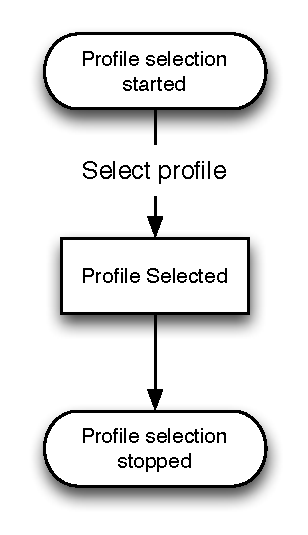
\includegraphics[width=0.3\textwidth]{gfx/profileselect_design.pdf}
	\caption{Features of the Profile selection feature}
	\label{fig:profileselection_design}
\end{figure}
The initial state of this feature is to choose which profile the previous selected should be launched as. This done by clicking on the chosen profile. If the chosen profile is not visible on the screen, it can be needed to scroll through the profiles in order to find it. When the chosen is clicked, the profile is selected and the profile selection process is over.
\section{QR code test}
To make a decision on how many characters the QR codes should hold it was needed to make a test. The test was done by making a timer on the device and see how long it would take to move the tablet from the table over the QR code to the authentication accepted. 
From what can be seen in the results it is not possible to make a comparison because it is such a small test size. But it can be concluded that there is no significant difference between using e.g. 10 and 200 characters. \\
The results from this test can be seen in \autoref{fig:QR-code-test}

\todo{should this be here?}
\section{GUI}
This section will explain the design decisions that was made considering the GUI in this produkt.

\section{Buttons and button design}
This section will explain the button design in the giraf system and how they were intended.

To make the overall consistency and usability better there were made some button guidelines. These were made to be used in the \giraf[] GUI library and thereby in the hole \giraf[] system including the launcher.

These guidelines included colors the buttons should have. The edge of the button should be a dark brown and the inner should be yellow and hereby the buttons are using the commen \giraf[] colors. Buttons should also have round corners if they are clickable and if they for some reason are not they should be squared. This can be seen in \autoref{fig:buttons}.

\begin{figure}[h!]
	\centering
	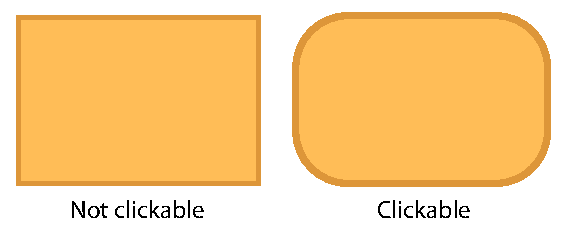
\includegraphics[scale=0.6]{gfx/buttons.pdf}
	\caption{Button illustration}
	\label{fig:buttons}
\end{figure}


\todo{Should this section be here?}
\subsection{Drawer}
\label{GUI:drawer}

The drawer is a feature where the user can hide tools when they do not use them or do not need them for a while. The drawer can be said to be some kind of toolbox. 

\subsection{The predefined colors} 
\label{GUI:colors}


Another reason was that it was important to control the functionality where the apps could use the same background color in the app as the icon background color. \\
If this was not done there could be problems like e.g. the user could set the icon background to white and if the icon was white then the user could not see what app it was and vice versa. Another problem could be that if the apps used the functionality where they can set the same background color in the app as the icon background color there could be none sufficient contrast. This would make it impossible for the user to see anything in the app.



% QR-codes can be scanned by a built-in camera on tablets and can be printed using standard paper and printer equipment. 
% 
% QR-codes are copyable, by e.g. a copymachine, and therefore must be kept away from untrusted users, if they should not be used by people for which they were not intended.
% 
% To sum up, QR-codes are chosen because of they improve usability, despite of their ability to be copied.\todo{Ulrik, er dette i orden?}
% 
% \begin{figure}[h]
% 	\centering
% 	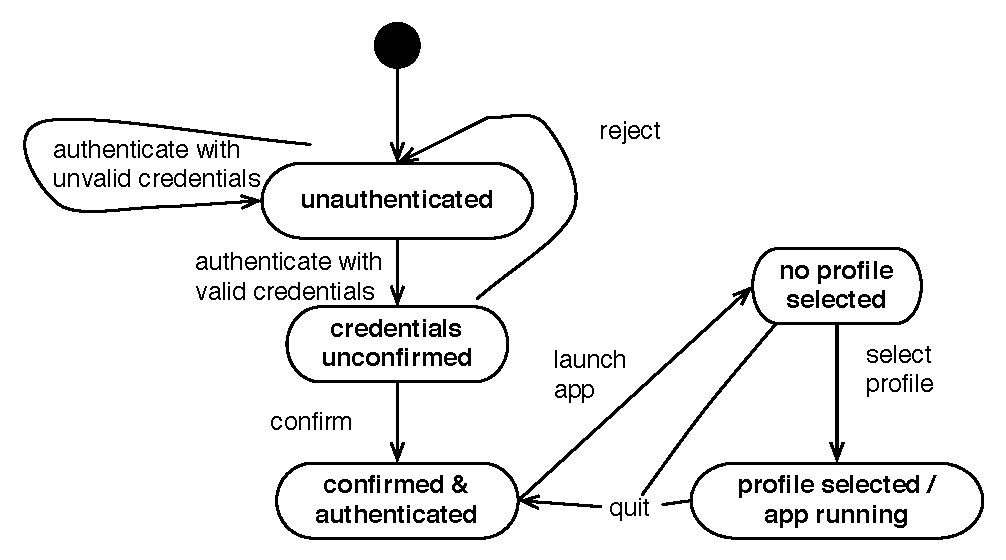
\includegraphics[width=1\textwidth]{gfx/flow-diagram2.pdf}
% 	\caption{Flow diagram}
% 	\label{fig:flow_diagram}
% \end{figure}
% 
% \autoref{fig:flow_diagram} shows the state of the launcher. The first three states handles the distinction between users which are allowed to access the launchable applications, and those who are not. \todo{indsaet ref til der hvor vi fandt ud af at vi skulle have authentication}
% 
% \begin{figure}[h]
% 	\centering
% 	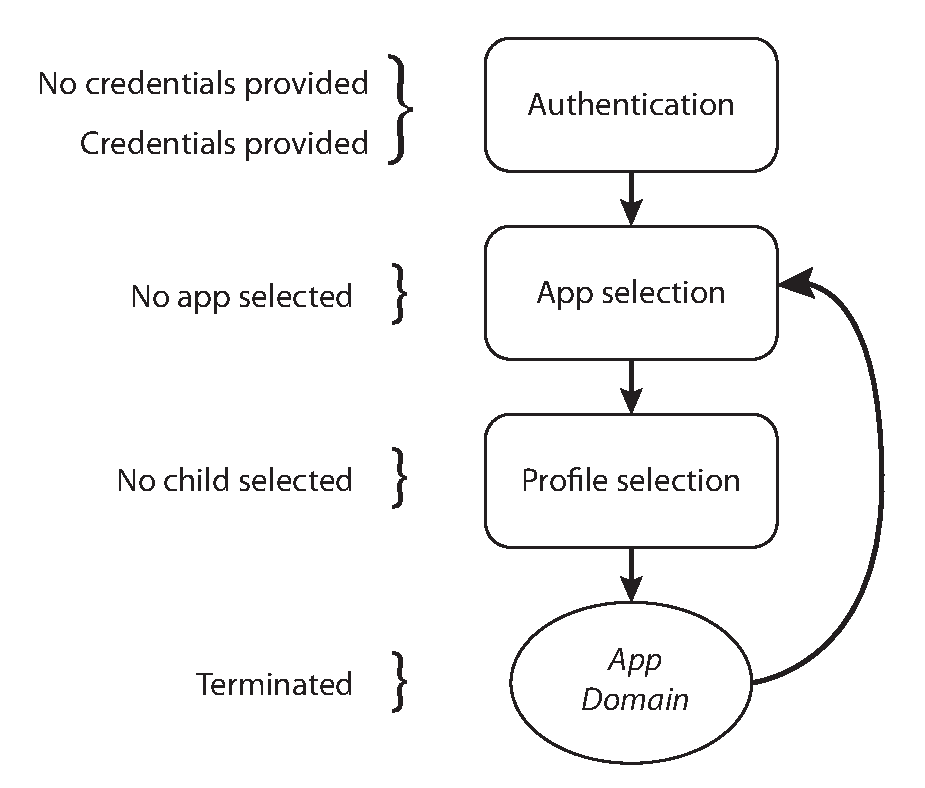
\includegraphics[width=1\textwidth]{gfx/design_diagram.pdf}
% 	\caption{Design diagram}
% 	\label{fig:design_diagram}
% \end{figure}
% 
% \begin{figure}[h]
% 	\centering
% 	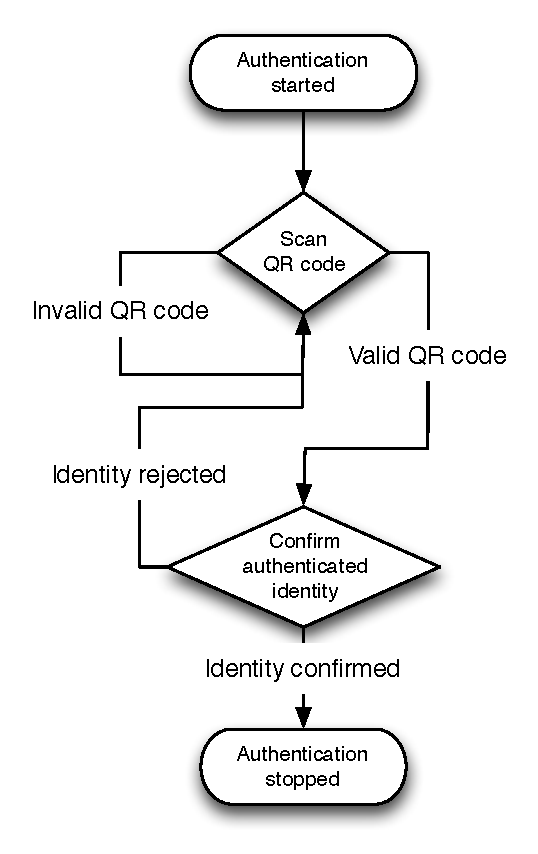
\includegraphics[width=0.5\textwidth]{gfx/authentication_design.pdf}
% 	\caption{Features of the Authentication functionality}
% 	\label{fig:authentication_design}
% \end{figure}
% 
% \autoref{fig:authentication_design} shows the states of the \activity{Authentication}. The simple ones is the start and stop states and they does just what they say. The interessting states is the ``Scan QR code'' state where when a user scans an QR code there is two path: One is that the QR code is invalid. The other one is if the QR code is valid then it leeds to another state where the activity checks the identity of the QR code scanned if it is not an known identity it is rejected else the \activity{Authentication} logs in the user and termintes.
% 
% \begin{figure}[h]
% 	\centering
% 	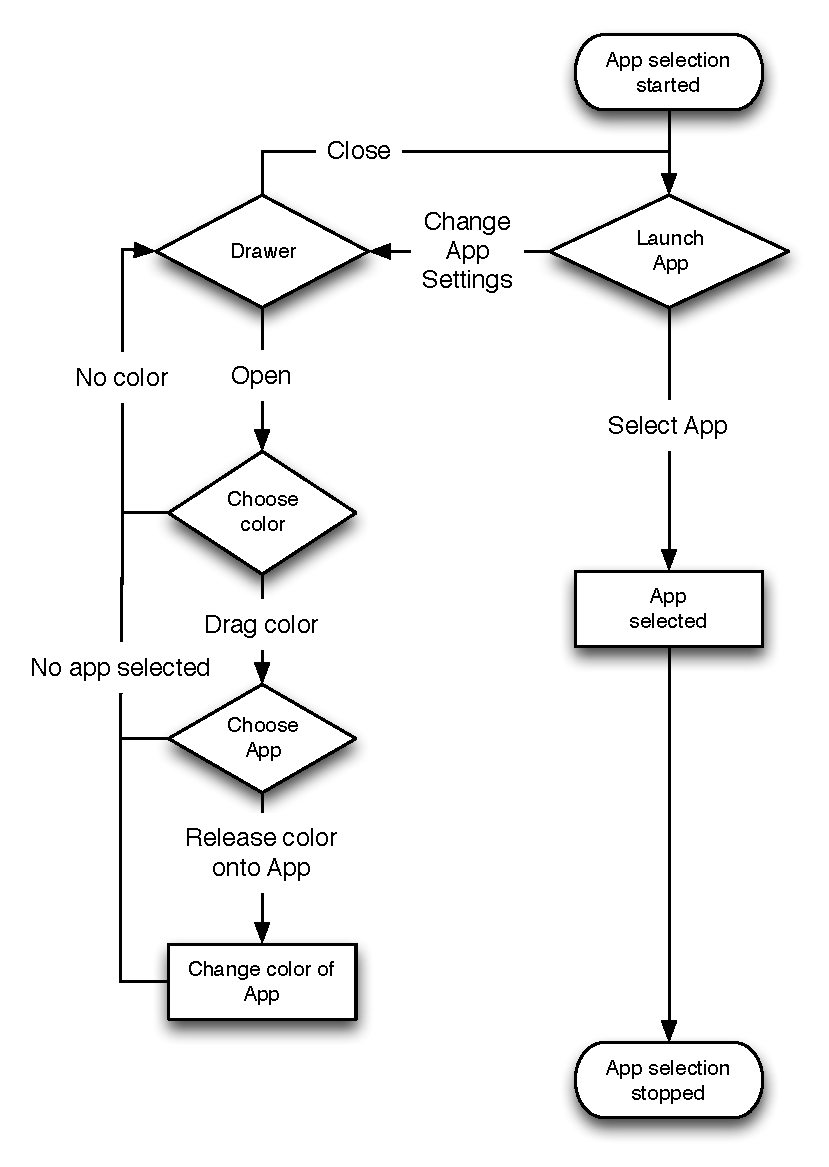
\includegraphics[width=0.7\textwidth]{gfx/appselection.pdf}
% 	\caption{Features of the App selection functionality}
% 	\label{fig:appselection_design}
% \end{figure}
% 
% \autoref{fig:appselection_design} shows the states that the app selection can take. 
% 
% \begin{figure}[h]
% 	\centering
% 	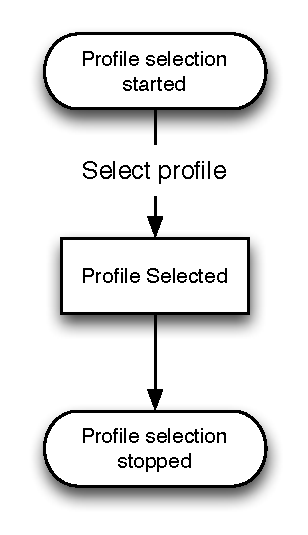
\includegraphics[width=0.3\textwidth]{gfx/profileselect_design.pdf}
% 	\caption{Features of the Profile selection functionality}
% 	\label{fig:profileselection_design}
% \end{figure}

%%%%%%%%%%%%%%%%%%%%%%%%%%%%%%%%%%%%%%%%%%%%%% COMMENT
\begin{comment}
Based on \autoref{fig:flow_diagram}, ..
\end{comment}
